% TEX root = ../Thesis.tex
\chapter{Introduction}
\newchapter{R}{esearch has shown that} climate change is a fact and that, with a 95\% certainty, human activity is the main cause for global warming \fcite{ipcc2013climate}. As a way to mitigate the increasing rate of climate change, the Danish government has set as an interim goal to reduce the national $CO_2$ emissions by 40\% in 2020, in order to reach the target of 80\% - 95\% reduction by 2050\fcite{regeringen2013danish}. This is to be done by covering 50\% of the national electricity consumption with wind energy by 2020, fully covering the electricity and heating supply with renewable energy by 2035, and being completely fossil fuel independent by 2050. Investing in an intelligent and flexible power system is deemed to be important if we are to reach those goals\fcite{regeringen2013smart}.

Aggregators of flexible consumption resources are expected to be a key element in the secure operation of power systems with large penetration of intermittent renewable energy sources. They will facilitate ancillary services to the system operators through the control of distributed flexible resources. Thus, traditional views on service specification, requirements, validation procedures and verification must be adapted to the new power system paradigm. 
%This will occur by providing services to the system operators through the control of the flexible resources.

The motivation for changing energy production to renewable sources is presented in Section~\ref{sec:justification}. A general description of the changes to the power system is presented in Section~\ref{sec:powsysdesc}. The technical problem formulation is presented in Section~\ref{sec:funneling}, where challenges are identified within this new power system framework, and this work's contributions to solve said challenges are summarized.
%adopted by the Danish government, a large part of Danish research has been focused on how to integrate renewable energy sources, as well as new distributed energy resources, into the power system. The world energy sector is experiencing drastic changes due to environmental, health and security issues. 
%% Clearpage necessary for B5 size
%\clearpage
\section{On the justification of research in renewable generation} % (fold)
\label{sec:justification}
\newsection{E}{nergy is a pillar} in the development of all countries. The access to energy is a necessity that traditionally is supplied by fossil fuels, but the use of fossil fuels carries consequences that have impacted nature and society in three different ways:
\begin{description}
	\item[Climate issues:] Reports like the Stern Review\fcite{stern2006stern} have made it abundantly clear that global warming and climate change will have considerable negative impact on society. If the current trend continues, global temperatures will rise 2-3 $^\circ$C within the next fifty years, but this number will increase by several degrees if emissions continue to grow. The consequences of global warming will impact society mainly through issues related to water:
		\begin{itemize}
			\item melting glaciers will increase flood risk and reduce water supplies
			\item declining crop yields
			\item rising sea levels will result in increased floods, as well as the disappearance of coastal regions and islands\footnote{According to one estimate, up to 200 million people may become permanently displaced due to these effects by mid-century\cite{stern2006stern}.}
			\item changes in ecosystems may lead to the extinction of 15 - 40\% of species, and the acidification of oceans may lead to decline in fish stocks
		\end{itemize}
	\item[Health issues:] Air pollutants resulting from the use of fossil fuel for transportation and electricity generation has been shown to be responsible for large numbers of morbidity and mortality. For example, in a study focused on traffic-related air pollution on public health in Austria, France and Switzerland\fcite{kunzli2000public}, it is found that in these three countries air pollution is directly attributable to:
		\begin{itemize}
			\item 6\% of total mortality (40 000 cases)
			\item 25 000 new cases of chronic bronchitis in adults
			\item more than 290 000 episodes of bronchitis in children
			\item more that 0.5 million asthma attacks
			\item more than 16 million person-days of restricted activities.
		\end{itemize} 
		Other sources\fcite{lelieveld2015a,who2014fact} estimate that air pollution leads to 3.3 - 3.7 million premature deaths per year, with the majority of the deaths occurring in Asia.
		Furthermore, climate change will have a direct impact on health through:
		\begin{itemize}
			\item increased frequency of and intensity of heat waves
			\item changes in distribution of vector-borne diseases
			\item increased floods and droughts\fcite{haines2006climate}
		\end{itemize}
	\item[Geo-political issues:] The concept of energy security has changed from being a local issue to include new concepts with respect to the provision of energy services. While traditionally it was a simple question of supply, measured by the four As of energy security (availability, affordability, accessibility and acceptability), it now encompasses concepts as efficiency, environmentally benign, properly governed and socially acceptable energy services\fcite{pasqualetti2012importance}. Also, governments around the world are taking steps to mitigate their vulnerability in energy supply, increasing the importance of sustainable energy generation. 
\end{description}

In the work by \textit{Cherp \& Jewel}\fcite{cherp2014concept}, the authors make a compelling argument for a new method for addressing the concept of \emph{energy security} by treating it as a case of general security. Thus, \emph{energy security} must address the questions: 1) \emph{Security for whom?}; 2) \emph{Security for which values}; and, 3) \emph{Security from what threats?}. Following the Danish government's climate policy plan and the goals of Energinet.dk\sidenote{Energinet.dk is the Danish Transmission System Operator, the entity responsible of maintaining a secure transmission power grid.}, these three question can be answered in a Danish context as:
\begin{enumerate}
	\item \emph{Energy security} in Denmark means that the population and industry should have an \emph{adequate} and \emph{secure}\sidenote{\emph{System adequacy} refers to the power system's ability to supply electricity demand at all times and \emph{system security} refers to the ability to withstand sudden disturbances \cite{entsoe2014glossary}.} power system.
	\item Given the previously cited climate policy plan, it is safe to assume that sustainability is the major value in what concerns \emph{energy security}.
	\item All the threats to \emph{energy security} can not be outlined here, but they include concepts of resilience and vulnerabilities. An example of a new vulnerability is the dependence on intermittent energy sources.
\end{enumerate}

In short, in order for the government to secure the future of the population against climate change, while ensuring that Denmark remains economically competitive through the research and export of green technologies, it is essential that a transition to a sustainable\fcite{brundtland1987our} energy system is achieved. 

This thesis addresses one of the solutions proposed to deal with the vulnerability introduced by the increasing penetration of intermittent renewable energy sources in the grid, as well as the increased stress on the power system due to the electrification of the transport and heating sectors. The following section explains the changes that the grid experiences as a consequence of the transition to a sustainable power system.
% section justification (end)
\section{Changes in the power system}% (fold)
\label{sec:powsysdesc}
\newsection{I}{n order to understand} the relevance of this research project, it is important to define how the power system is expected to change, and clarify the frame for the research. This section gives a general introduction %\footnote{In-depth explanations will be presented as needed in subsequent chapters.} 
 to the changes expected in the power system. The main actors in the power system and their relationships (from a Danish perspective) are presented, which will help scoping the problem.%\marginnote{This section is based on an unpublished paper written for the course 31920, Communicating Advanced topics in Electrical Engineering.} 
\subsection*{The Traditional Power System: Produce as we Consume}
\label{sub:traditional}
\marginnote{This subsection is intended for readers who are not already familiar with the power system. It clarifies basic concepts such as production/consumption balance, system frequency, system operators, energy markets, etc.}
The goal of the power system is to provide an adequate and secure electricity supply to the population.
The electric power system today is composed of two layers (Figures~\ref{fig:powernow}-\ref{fig:marketnow}): 
\begin{description}
	\item[Physical grid] This is the level at which the electricity flows, going from generators to transmission system, to distribution system and finally to the end consumer.
	\item[Market layer] This is where all the energy trade and business operations are made. This includes the sale of electricity from producers to \glspl{brc}. Retailers in turn buy electricity from the BRCs and sell it to the end consumer. Being a \gls{brp}, either as a consumer or as a producer, means that the actor is responsible for its own forecasts and must ensure the best possible that the actual production/consumption follows the planned schedules.
\end{description}

\begin{figure}[t]
	\centering
	\caption{The Electric Power System as seen today. The power generated is first transmitted at high voltage levels to industrial consumers and transformer substations, from where it is distributed at medium/low voltage to medium size consumers and households.}\label{fig:powernow}
	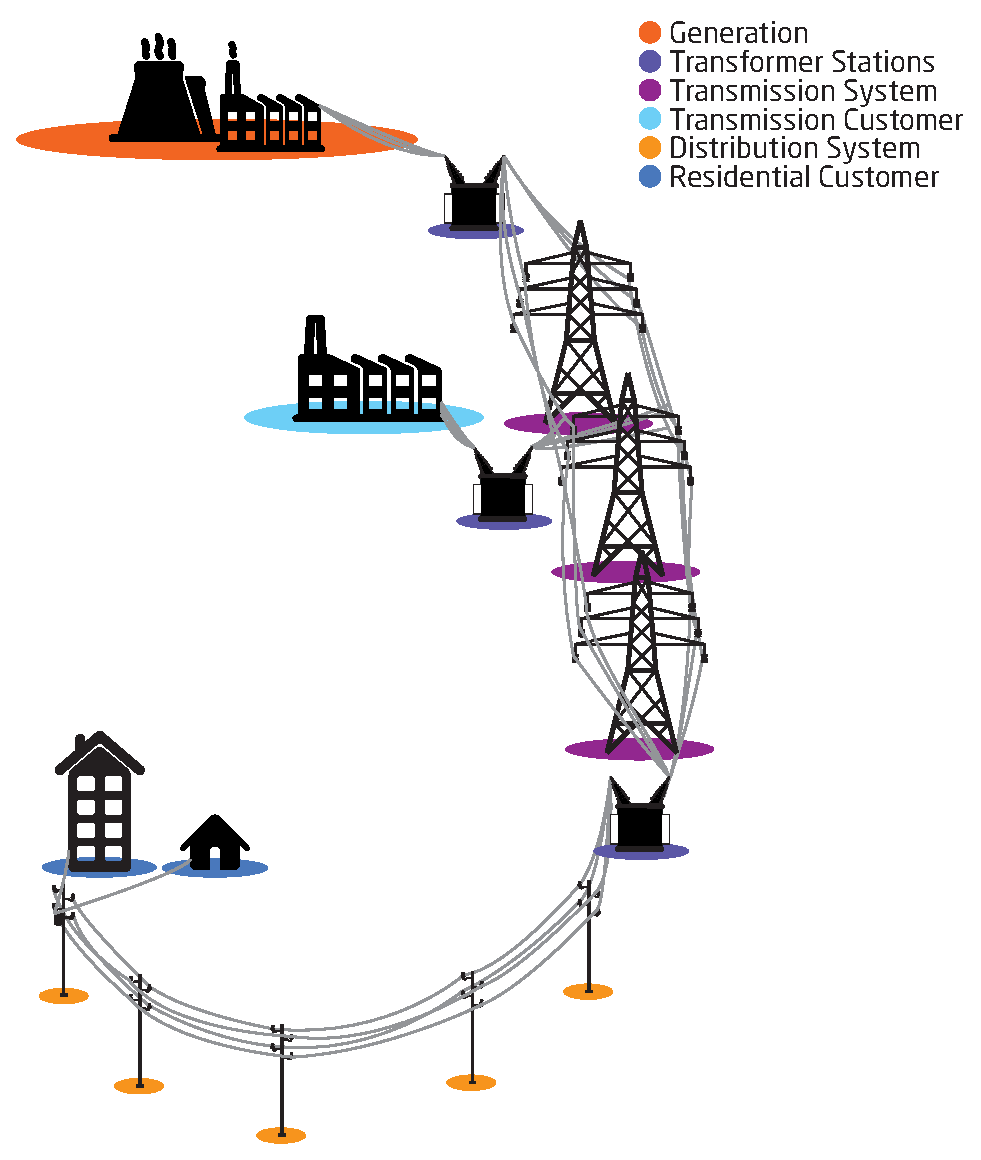
\includegraphics[width=\textwidth]{intro/traditional_grid_new.eps}
\end{figure}

While market regulations can be adjusted or completely changed in order to cope with the large influx of renewable energy, the physical laws cannot.
When electricity is produced it must also be consumed. With current technology it is unfeasible to store electricity in large quantities, therefore electricity companies must forecast how much electricity consumers are going to need the next day and then buy electricity accordingly. I.e., the production of electricity must match the consumption of electricity. If there is a surplus of electricity in the system (production exceeds consumption), the system frequency increases\sidenote[][-3\baselineskip]{The system frequency is a measure of the balance of the grid. Electricity is traditionally produced with turbines which rotate synchronously in a given area. The system frequency, e.g. 50 Hz in Europe, is a measure of the balance of the system, with higher frequencies signaling a power surplus and lower frequencies signaling power deficit in the system.}%\todo{Check up on sources}}
, and might eventually damage electric components in the grid. Vice versa, a deficiency of electricity in the system (consumption exceeds production) can lead to a blackout. 
\begin{figure*}[htbp!]
		\centering
		\caption{The actors and relationships in the power market today. Note that the consumer buys electricity from a retailer, but has no further contact to the other market actors, i.e. the consumer has a passive role in the system.}\label{fig:marketnow}
	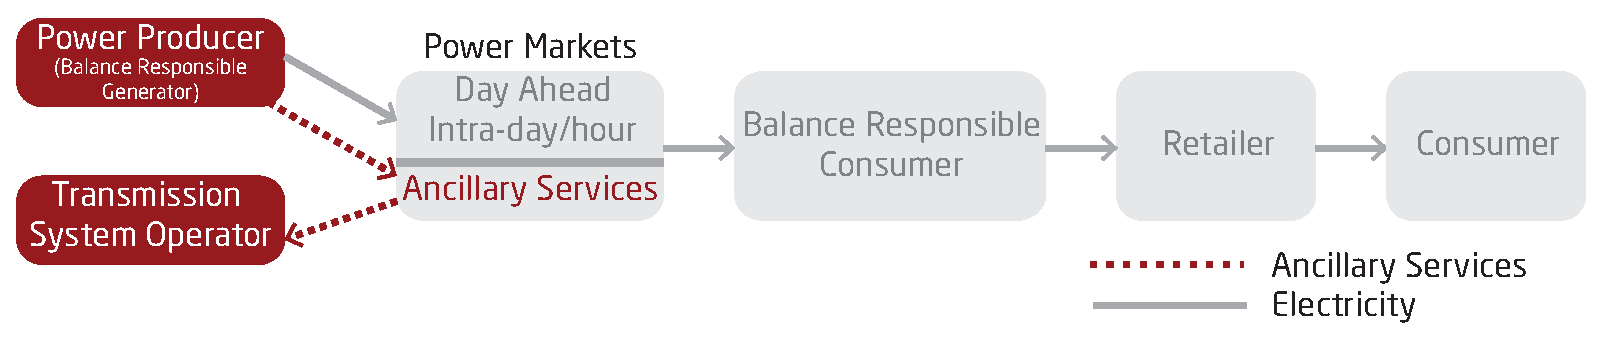
\includegraphics[width=0.8\textwidth]{intro/market_now.eps}
\end{figure*}

The consumption forecasts are imperfect, which leads to a constant imbalance between production and consumption of electricity. The \gls{tso} is the entity responsible of resolving the imbalances of the system and maintaining the secure operation of the system. In order to do this, the TSO buys ancillary services from \emph{certified generators}\footnote[][-2\baselineskip]{The concept of certification of units to deliver ancillary services is central to this work and will be expanded upon in Chapter~\ref{cha:validation}.}  through the ancillary service markets. This market relationship is also reflected in Figure~\ref{fig:marketnow}. There are different types of services, and thorough overviews and explanations of these can be found in the literature\fcite{entso1operational,Rebours}. Here it suffices to say\footnote{Further discussion on ancillary services will be presented in Chapter~\ref{cha:services}.} that for most ancillary services, the TSO will pay generators to deviate from their planned production plans in order to bring the system back to balance. In the future, it is expected that the traditional sources of ancillary services, i.e. large central fossil-fuel powered generation plants, will be outphased in favor of smaller distributed and renewable generation. This means that new sources for ancillary services must be found.  

\subsection*{The New Flexible Power System: Consume as we Produce}
\label{sub:future}
In the traditional power system, the uncertainty in consumption causes imbalances. With the increase of wind energy and solar generation, the uncertainty traditionally only associated with consumption spreads to the production side. Furthermore, traditional sources of ancillary services are closing down, which means that TSOs must find new ways of balancing the system. Also, new problems will appear at the distribution system level, such as power congestion and voltage issues. These problems arise because of new consumption technologies appearing in the system, such as \glspl{ev} and \glspl{hp}, and because of new generation units, \eg \glspl{wt}, small size \glspl{chp} and \glspl{pv}, are installed at distribution level. All these new units in the electric power system are commonly referred to as \glspl{der}\footnote{In this work the concept of DER includes \gls{dg}, \gls{ee}, demand response (DR) and \gls{dess}, which is a combination of the the traditional definition of DER = DG + DESS (as seen in \eg \cite{nrel2002using}) and the broader definition presented in \cite{nys2014reforming}.} or flexible resources. It is the responsibility of the \gls{dso} to resolve the problems arising due to the integration of the DERs, which can be the overloading of system components or voltage issues. These problems affect the quality of the power supply at residential level, but can also lead to issues at transmission level.
\begin{figure}[ht]
	\centering
	\caption{The Electric Power System of tomorrow contains a large ICT infrastructure, which permits the flow of information and control between the system actors. Furthermore, the flow of electricity is not only from generator to consumer, but there is also intermittent electricity generation at distribution level.}
	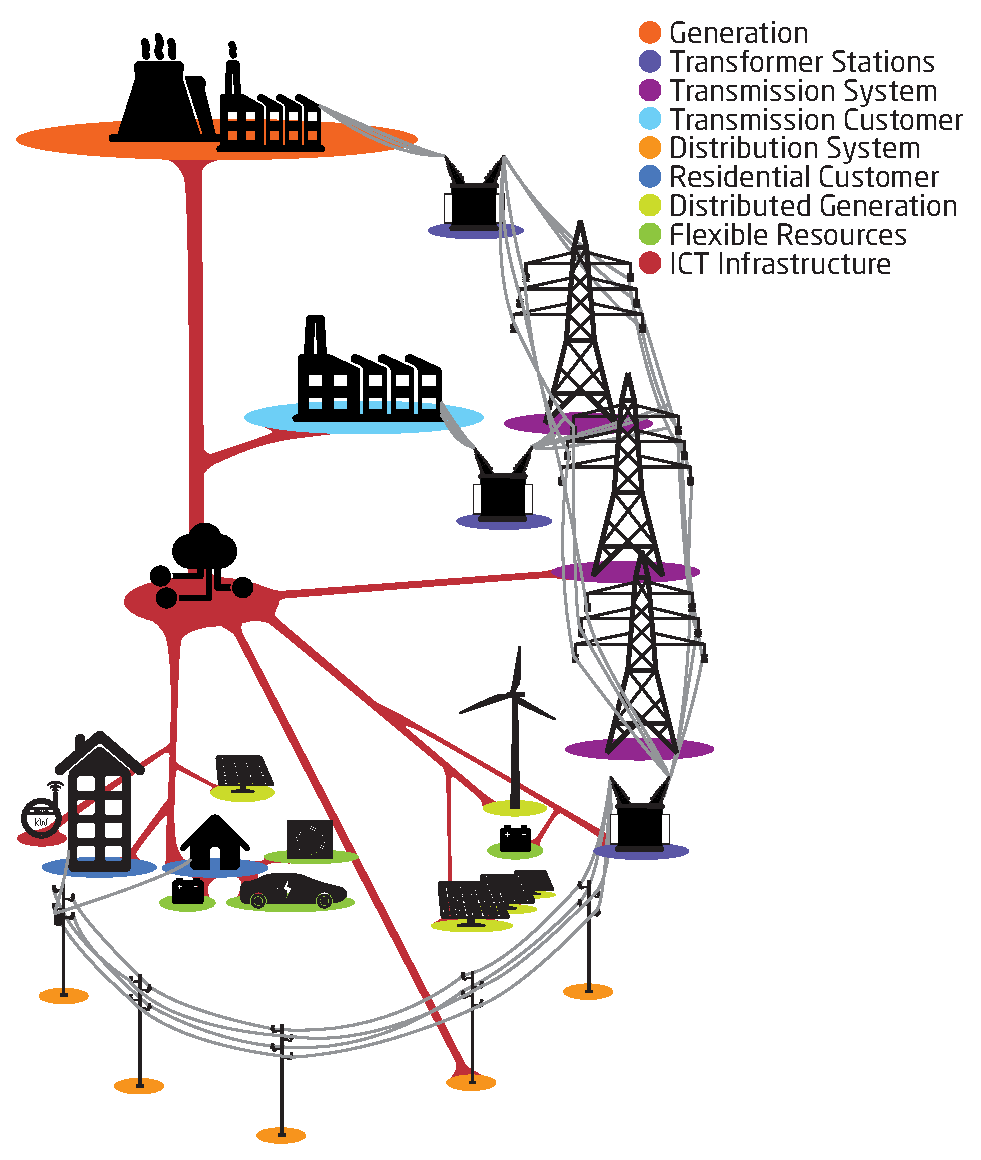
\includegraphics[width=\textwidth]{intro/smart_grid_new.eps}\label{fig:powerfuture}
\end{figure}

The expected future smart grid can be seen in Figure~\ref{fig:powerfuture}, where not only the new DERs appear but an \Gls{ict} infrastructure coordinates the behaviour of the units for the benefit of the system. Smart metering is added at consumer level, and sensors are deployed at distribution level.
\begin{figure*}[htbp!]
	\centering
	\caption{The actors and relationships in the power market of tomorrow. Compared to the current market setup, the aggregator entity has been added, as well as the ability of DSOs to contract services from the aggregator. The aggregator delivers ancillary services to the TSO through a BRC. Also, the consumer becomes a player in the electricity markets through the aggregator.}
	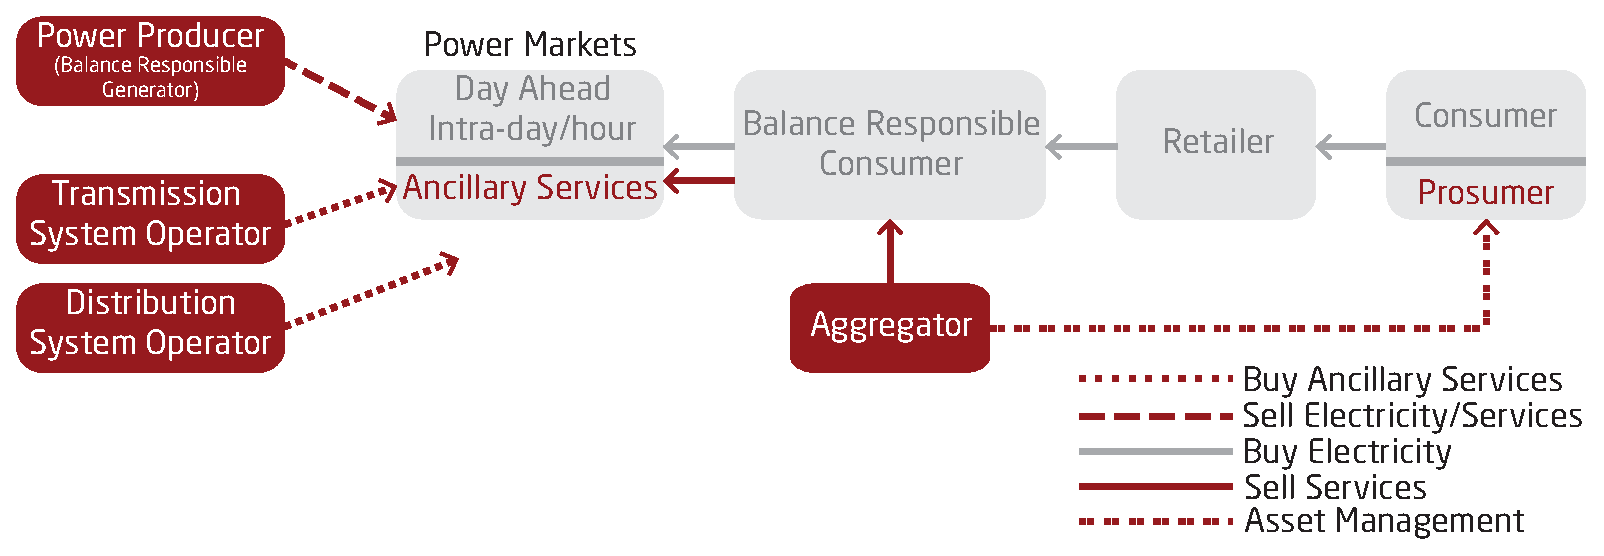
\includegraphics[width=0.8\textwidth]{intro/market_future.eps}\label{fig:marketfuture}
\end{figure*}

In order to cope with the new problems, both at transmission and distribution level, it is expected that consumers will become prosumers. That is, the consumers will take an active role in the power markets by selling services to the system operators through an aggregator\footnote{The concept of the aggregator is further discussed in Chapter~\ref{cha:aggregator}.}. The aggregator will provide an asset management service to the end consumer, and by managing a pool of consumers, it will be able to control a large enough consumption volume to provide ancillary services to the system operators, or balancing services to the consumption BRP. The action of a consumer changing his or her consumption based upon an incentive is known as \gls{dr}. The aggregator facilitates DR by providing the ICT infrastructure and control infrastructure to DER owners, as well as statistical certainty of service delivery and legal responsibility towards the system operators. The aggregator can be an independent commercial entity, or it can be a function inside one of the pre-existing market players. The new market setup can be seen in Figure~\ref{fig:marketfuture}, and it shows how the aggregator entity will interact with the existing market setup, and how the DSO will become a new player in the market, which will acquire services to resolve some of it problems.

In conclusion, we see the electric power system moving away from a \emph{production-must-follow-consumption} pattern to \emph{consumption-should-partly-follow-production} and hereby facilitate the integration of renewables and DERs. An integral part of achieving this change will be the use of control services to change the consumption behavior of units in the network. Given that the units providing ancillary services to the grid are critical for the security of the system, system operators must be able to trust that the units will behave as required. This is ensured by validating the new control algorithms and infrastructure through tests.



%\todo{amplify the paper to contain an analogy of the frequency as inflow and outflow of a water tank}
% section Short introduction to the power system (end)

\section{Problem statement, Delimitation and Contributions} % (fold)
\label{sec:funneling}
\newsection{A}{ggregators are expected to} be new providers of ancillary services to the Transmission System Operators and flexibility services to the Distribution System Operators and Balance Responsible Parties by means of controlling flexibility. They must go through the same prequalification/certification process that current providers of ancillary services must go through. Therefore, the control algorithms and architecture that form an aggregator must be validated\marginnote{The Institute for Electrical and Electronics Engineers (IEEE) defines validation as: ``The assurance that a product, service, or system meets the needs of the customer and other identified stakeholders.''}. Several factors, such as the distributed nature and the modular composition of aggregators, make this problem non-trivial. The overarching question this thesis seeks to answer is: \emph{How can aggregators be validated, such that they can be trusted by the power market participants, and hereby actively help with the secure operation of the power system?}.

Considering that \emph{validation} is the key word in this question, the overarching question can be split into the following subproblems:
\begin{enumerate}
	\item what are the needs the TSO wants fulfilled when acquiring services?
	%\item can an aggregator fulfill those needs?
	\item how can we measure how close the aggregator is to fulfilling those needs?
	\item how can we establish a systematic procedure for assuring that the aggregator matches the required needs?
\end{enumerate}
%control-services? This is a broad definition, and here I will  narrow down my research to use control services to provide ancillary services, primarily through demand response, but the techniques should be able to be generalized.

\subsection*{Scoping and Methodology}
%In order to delimit the scope of the problem, certain decisions with regards to the research were made.
The operation of the power system varies widely between countries and the scope of ancillary services is wide. This thesis limits its focus to the following:
\begin{itemize}
	\item In terms of the services considered, only those related to active power were analysed. The topic of voltage related services was touched upon as a collaboration with \emph{X. Han et al.}\fcite{han2014assessment}, but does not form part of the core of the presented research.
	\item The power system setup is assumed to be a liberalized market, such as the one in Denmark. Although some of the work is translatable to other countries, e.g. the United States, the focus has been on solutions suited to the Nordic region.
\end{itemize}

The methodology that has been followed has been pragmatic in nature. An understanding of the TSOs' empirical solutions to these problems has been achieved through the analysis of the regulations of Energinet.dk (the Danish TSO), the \gls{entsoe} and PJM (an American \gls{rto}), as well as through email correspondence and telephone interviews with representatives of Energinet.dk, PJM and CAISO (the Independent System Operator (ISO) of California). Parting from the status quo, for each research subquestion an analytical approach to identifying future requirements was taken, and a systems engineering approach in collecting these requirements. Solutions were designed with these requirements as goals or constraints.

\subsection*{Contributions}
%Focus has been given to the development of concepts rather than software implementation. Still, a module for service verification was developed for the laboratory.
The original contributions to the field are:
\begin{description}
	\item[Aggregator reference architecture:] The analysis of the aggregator in the power system through concepts from computer science and system engineering. Chapter~\ref{cha:aggregator} presents a candidate reference architecture for aggregators, which has the purpose of:
		\begin{enumerate}
			\item defining a standard lexicon around the aggregator, and
			\item identifying the required functionality necessary for the effective working of an aggregator.
		\end{enumerate}
		These two points are essential for understanding how the aggregator can fulfill the TSO needs.%\footnote{ The reference architecture can also be used as aggregator design guidelines for new players entering the market.}. 
	\item[Aggregator validation procedure:] Validation methods for large central generation units are well developed, but must be adapted for aggregators of large quantities of small-scale distributed resources. The contribution is the expansion of the traditional method of validating generators to include statistical measures for service requirements and performance, as well as statistical test design methods to the validation test procedure. Chapter~\ref{cha:validation} presents a framework for aggregator validation testing, as well as the outline of a procedure for validation tests. This contribution is important because it ensures capabilities of the aggregator are adequate for service provision.
	\item[Definition and modeling of services:] Currently, the requirement definitions for ancillary services assume that the services will be provided by traditional units. In Chapter~\ref{cha:services} a novel approach to ancillary service definitions is presented. Furthermore, a method for modeling service performance requirements was developed in order to facilitate service verification of aggregators. These contributions are important for the aggregator being able to deliver services in the power markets.
		 %The new ancillary service definition is necessary for effectively integrating aggregators, and other new technologies, into the power system as new sources of ancillary services. The method for service modeling provides the service models required for calculating performance assessment of aggregators, or other service providing technologies.
	\item[Aggregator performance assessment:] In order to verify if an aggregator delivered a service according to its service contract, the performance of the aggregator must be assessed. In Chapter~\ref{cha:verification} concepts from Control Performance Assessment, \ie from the field of process control, have been applied to the aggregator performance evaluation. This has resulted in a set of indices for performance assessment and service delivery are presented. These indices are general measures for service delivery and are novel in the way that they are not defined for specific services, but can be applied interchangeably to the service models defined in Chapter~\ref{cha:services}.
\end{description}

\subsection*{Thesis Structure}
Each chapter contains the relevant state-of-the-art analysis to that topic and corresponding sub-conclusions. The thesis focuses on the theoretical concepts presented in the publications, but most of these concepts have been illustrated through cases studies in the articles. Most of these case studies are not presented within the body of the thesis, but the reader can refer to the relevant articles in the appendices for said case studies.

Chapter~\ref{cha:aggregator} discusses what an aggregator is and Chapter~\ref{cha:validation} presents the work on aggregator validation. Chapter~\ref{cha:services} presents the work on services modeling and definition and Chapter~\ref{cha:verification} presents work on service verification and aggregator performance assessment. Overall conclusions and perspectives on future work are presented in Chapter~\ref{cha:conclusion}, and the relevant articles forming the research content of the thesis are found as appendices. 
%What is meant with control services? In european context it is very much focused on Ancillary Services, while in the US Demand Response has not been used very much as AS, but rather used by ISOs as a mechanic to cope with peak consumption, or in the wholesale market. In the US context it would not make sense to call the upward service for the aggregator an ancillary service. Maybe aggregator business case?

%``futures necessarily belong to the present: they are what we imagine for ourselves now. The present is itself only made visible against a past''[cite: Marilyn Strathern, 1992]

% section Funneling (end)


